\documentclass[a4paper]{article}

\usepackage[english]{babel}
\usepackage[utf8x]{inputenc}
\usepackage{amsmath}
\usepackage{amsfonts}
\usepackage{amssymb}
\usepackage{graphicx}
\usepackage{aaai}
\usepackage{fullpage}
\usepackage{listings}
\usepackage{float}
\usepackage{bbm}
\usepackage{wasysym}
\usepackage[colorinlistoftodos]{todonotes}
\usepackage{algorithm}
\usepackage{algpseudocode}
\newenvironment{courier}{\fontfamily{pcr}\selectfont}


\title{Planning with Affordances}
\author{Dave Abel and Gabriel Barth-Maron \\ \\ Department of Computer Science, Brown University \\ \\ \begin{courier}\{dabel,gabrielbm\}@cs.brown.edu\end{courier}}
\date{}


\begin{document}
\maketitle

\begin{abstract}
We introduce a novel approach to planning that combines the concept of affordances \cite{Gibson} with a standard planning algorithm, Value Iteration. Classical planning algorithms suffer from combinatoric state-space explosions \cite{Norvig} that cripple their effectiveness. Thus, in order to fully realize the potential of planning algorithms, we have sought to make these previously difficult problems more tractable; through the use of our affordance framework we seek to ``guide" the agent as it plans, significantly reducing the size of exponential state-spaces. To accomplish this, we propose a planning algorithm that prunes the state action space using affordances. Evaluation is performed in the Minecraft domain on several path planning tasks - we demonstrate a significant increase in speed and reduction in state-space exploration across 5 different path planning tasks.
\end{abstract}

\section{I. Introduction}
% Motivation
As robots move out of the lab and into the real world, planning algorithms need to be able to scale to domains of increased noise, size, and complexity. In Norvig and Russell's AI textbook, they state that, ``Planning is foremost an exercise in controlling combinatorial explosion." \cite{Norvig}, an explosion which is currently uncontrolled across many planning domains. A classic formalization of this issue is the sequential decision making problem, where increases in problem size and complexity directly correspond to an explosion in the state-action space. Current approaches to solving sequential decision making problems cannot tackle these problems as the state-action space becomes large \cite{Grounds2005}. 

There is a strong need for a generalizable form of knowledge that, when coupled with a planner, is capable of solving problems in these massive domains. Humans provide an excellent existence proof for such planning, as we are capable of searching over an immense number of possible actions when presented with a goal - a recent concept out of 20th century psychological literature, an ``affordance" has provided an explanation as to how this mechanism of human planning works.

% Affordance paragraph -- Flush this out
Broadly, an affordance is "what [the environment] offers [an] animal, what [the environment] provides or furnishes, either for good or ill" \cite{Gibson}, and may be employed in the context of planning to direct an agent toward relevant actions or parts of the environment (based on the agent's desires/goals). Additionally, roboticists have recently become interested in leveraging affordances for a variety of applications \cite{Koppula2013a} \cite{Koppula2013b}. In this paper we will employ affordances as a means of reducing large and intractable search problems into smaller, more reasonable problems. When instantiated in a physical robot, this will enable the robot to handle tasks that involve high order action spaces and expansive domains.

We propose a new formalism for representing affordances in an operationalized knowledge base. Current approaches to scaling MDPs up to large domains involve either pruning the state space of the world (by using subgoals), or limiting the action space \cite{Branavan2012}. In our approach, by introducing the affordance knowledge, we effectively limit the state space {\it and} the action space.

% Evaluation
We evaluate our method in a number of scenarios in the world building game Minecraft, and compare results against a classical Reinforcement Learning Planning Algorithm. Our results indicate that our affordance knowledge enables planning algorithms to scale to scenarios of arbitrary size and complexity, while our baseline cannot handle increased complexity in the state or action space. 

\begin{figure*}[t!]
\centering
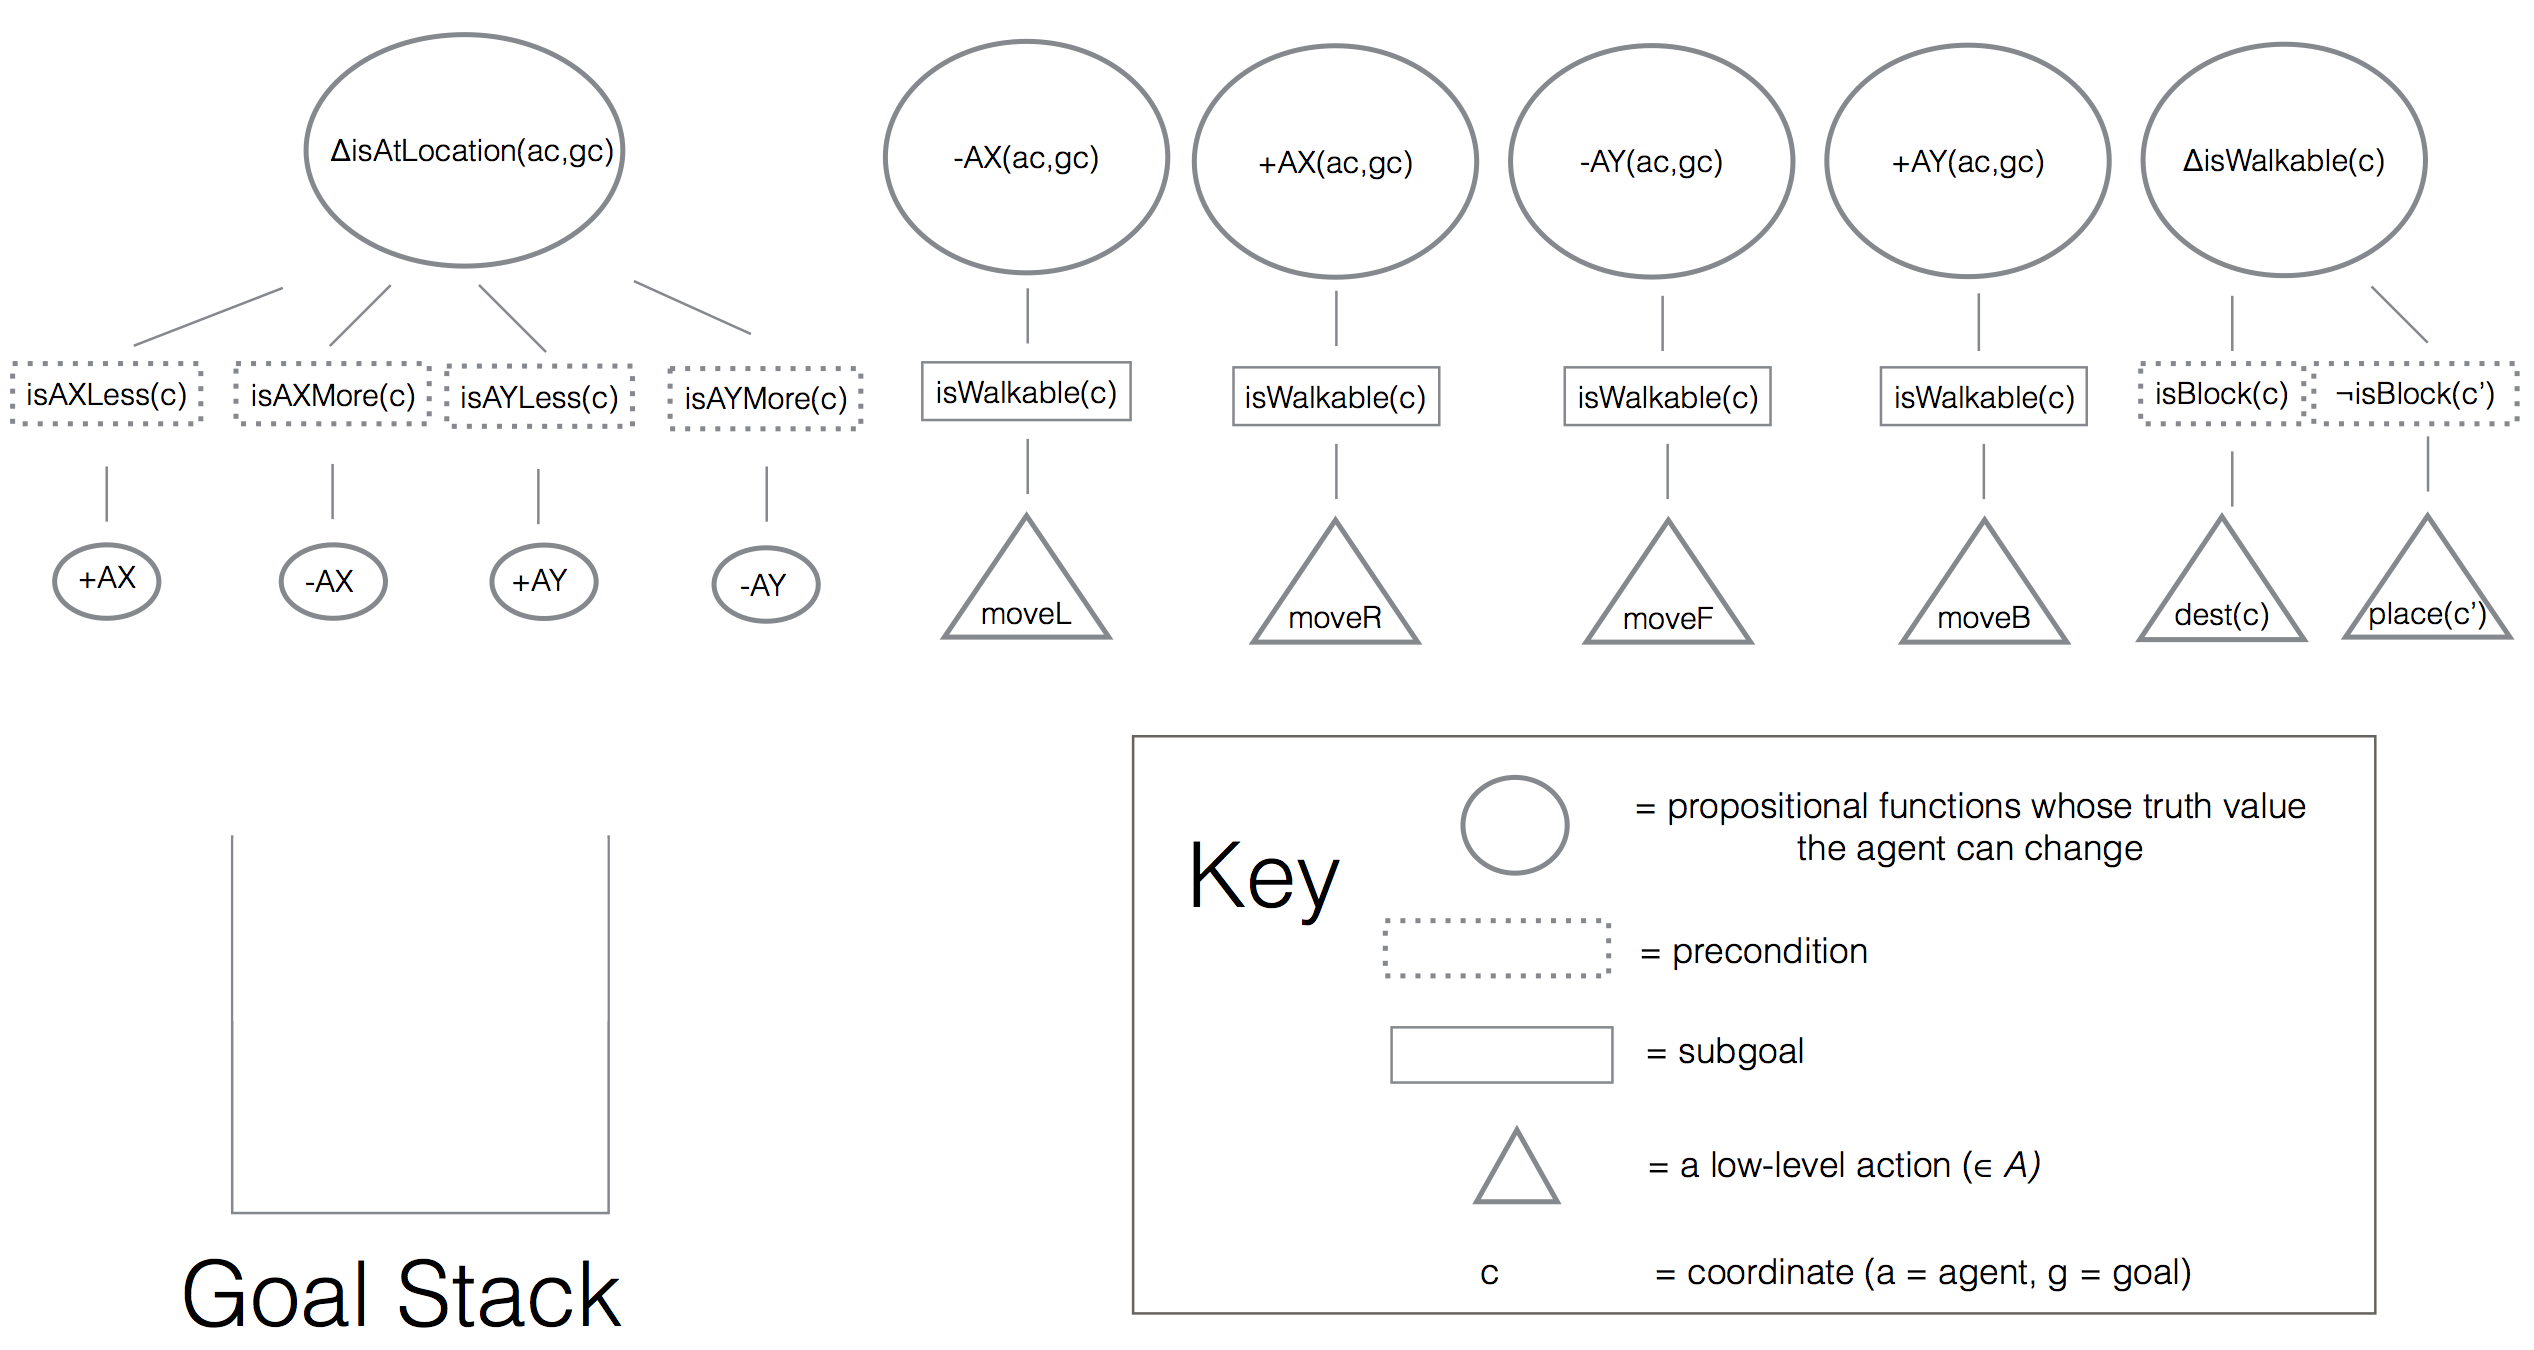
\includegraphics[scale=0.34]{images/formalism.png}
\caption{An example of the affordance-based knowledge formalism, geared toward path-planning problems}
\label{fig:affordance_tree}
\end{figure*}

\section{II. Related Work}
There have been several previous attempts at improving planning to handle the complexity of the sequential decision making task in large environments. \cite{Grounds2005} recently proposed incorporating a STRIPS planner with Value Iteration in order to overcome the shortcomings of classical VI. They demonstrated that Value Iteration could not handle reasonably complicated domains, and showed that their STRIPS \& VI planner was able to do slightly better. However, they did not scale the complexity and size of the domain up enough to indicate that their algorithm would generalize.

As mentioned above, one approach to making massive domains (large state-action space) more tractable for MDPs was to prune the search space. Past attempts at state-space pruning have focused on introducing subgoals as a means of narrowing the search space. Branavan et al. \cite{Branavan2012} learns preconditions for a Minecraft-like world by performing Information Extraction on the Minecraft Wiki page, and searching through the resulting high level precondition relations as a means of planning. This proved to be extremely effective for the set of tasks they visited in their paper.

However, we hypothesize that by only narrowing the state-space, it is not possible to scale planning on a massive level, and to generalize to different problem types. Our intuition is that introducing subgoals to the planning space narrows search, but often subgoal planning does not eliminate useless parts of the search space.

Further, we believe that our methodology, when equipped with the proper affordance knowledge, should be able to solve the various scenarios presented in \cite{Branavan2012}. On the other hand, movement based tasks such as the ones we visit in this paper are difficult to do with only subgoal search - this is because subgoals do not map onto most movement-based goals effectively.

Mark Steedman has done quite a bit of work with Affordances \cite{Steedman2011} \cite{Steedman2002}. Most notably, he introduced the Linear Dynamic Event Calculus (LDEC) which served as heavy inspiration for our own formalism. The LDEC was not created with subgoal planning in mind, which is why we chose to use it as motivation, and not explicitly as part of our planning algorithm.

Additionally, as mentioned before, the robotics community has become interested in affordances - Koppola and Saxena used affordances to anticipate human actions as well as predict human poses in a room \cite{Koppula2013a} \cite{Koppula2013b}, and Andreas ten Pas \cite{Pas} leveraged affordances to improve robotic grasping ,  just to name a few.

There is also a subfield of planning known as Partial Order Planning, that saw a large growth in popularity during the 80s and 90s, but lost much of its following at the turn of the millenium \cite{Norvig}. The gist of Partially Ordered Planning is that it uses a list of ordered subgoals in order to solve a problem. There are several reasons that POP lost its favor in the planning community, but the primary one seems to be that it did not fundamentally solve the state-space explosion problem; it simply moved the search problem to searching over subgoals. There have been a few attempts to revive POP over the years \cite{Nguyen2002}, but have not proven ultimately successful.

\section{III. Background}

\subsection*{Affordances}

An affordance is what an environment, or the objects in it, offer the agent. For example, if the agent were trying to drink coffee then a mug would afford carrying liquid. However if instead the agent wanted to secure some papers outside on a windy day, then the mug could afford weighing the papers down (i.e. affords using it as a paper weight). Often, objects may be defined in terms of what they afford, such as a bridge - suppose there is a log lying horizontally across a river; such a log provides passage over a river and could reasonably be referred to as a "bridge" simply because it affords crossing the river.\footnote{There is a compelling and as of yet (by these authors) unexplored relationship between language and affordances - this is an area we would like to delve in to with our formalism in the future}

\subsection{Minecraft}

We chose to evaluate our algorithm in the context of the world building game, Minecraft, which serves as an excellent domain due to its high degree of complexity and flexibility. We were able to interact directly with the Minecraft world due to the recent development of the Mineflayer Bot API \cite{Mineflayer}. 

There are a number of compelling categories of plannings tasks available in such a world, including basic path planning, object building, tool construction, and many more. For our purposes, we will be focusing on path planning tasks, though we feel confident that our algorithm should generalize to other types of planning problems given the right affordance knowledge. One primary extension of this project is to test our algorithm across a variety of tasks.

\section{IV. Problem Statement}

The standard MDP planning algorithm, Value Iteration, is only useful in small, simple domains \cite{Norvig} \cite{Grounds2005}. Any instance in which the state-action space grows beyond a certain threshold causes serious problems, as Value Iteration has to enumerate the entire state space. This is a massive problem, and seems intuitively strange for any sort of planning, as the majority of states in many planning domains are completely unrelated to the goal, and any reasonable agent would never even consider them. For instance, if a human agent were trying to exit a library, their strategy would not involve reading every book on the way to the exit (the agent would long exceed their lifespan prior to reading all books in a library) - these actions (reading books) do not contribute towards reaching the goal, in this case. So, it seems reasonable that in the case of Value Iteration, we should be able to rid ourselves of enumerating a huge number of states that don't relate to the agent's current goal.

Fundamentally, the intuition behind our algorithm is that there are many states that do not need to be explored, and furthermore, many actions that are useless in a number of states. Affordance knowledge capitalizes on this assumption by directing the agent toward relevant states and actions that lead the agent toward its goal.

\begin{figure*}[t!]
	\centering
	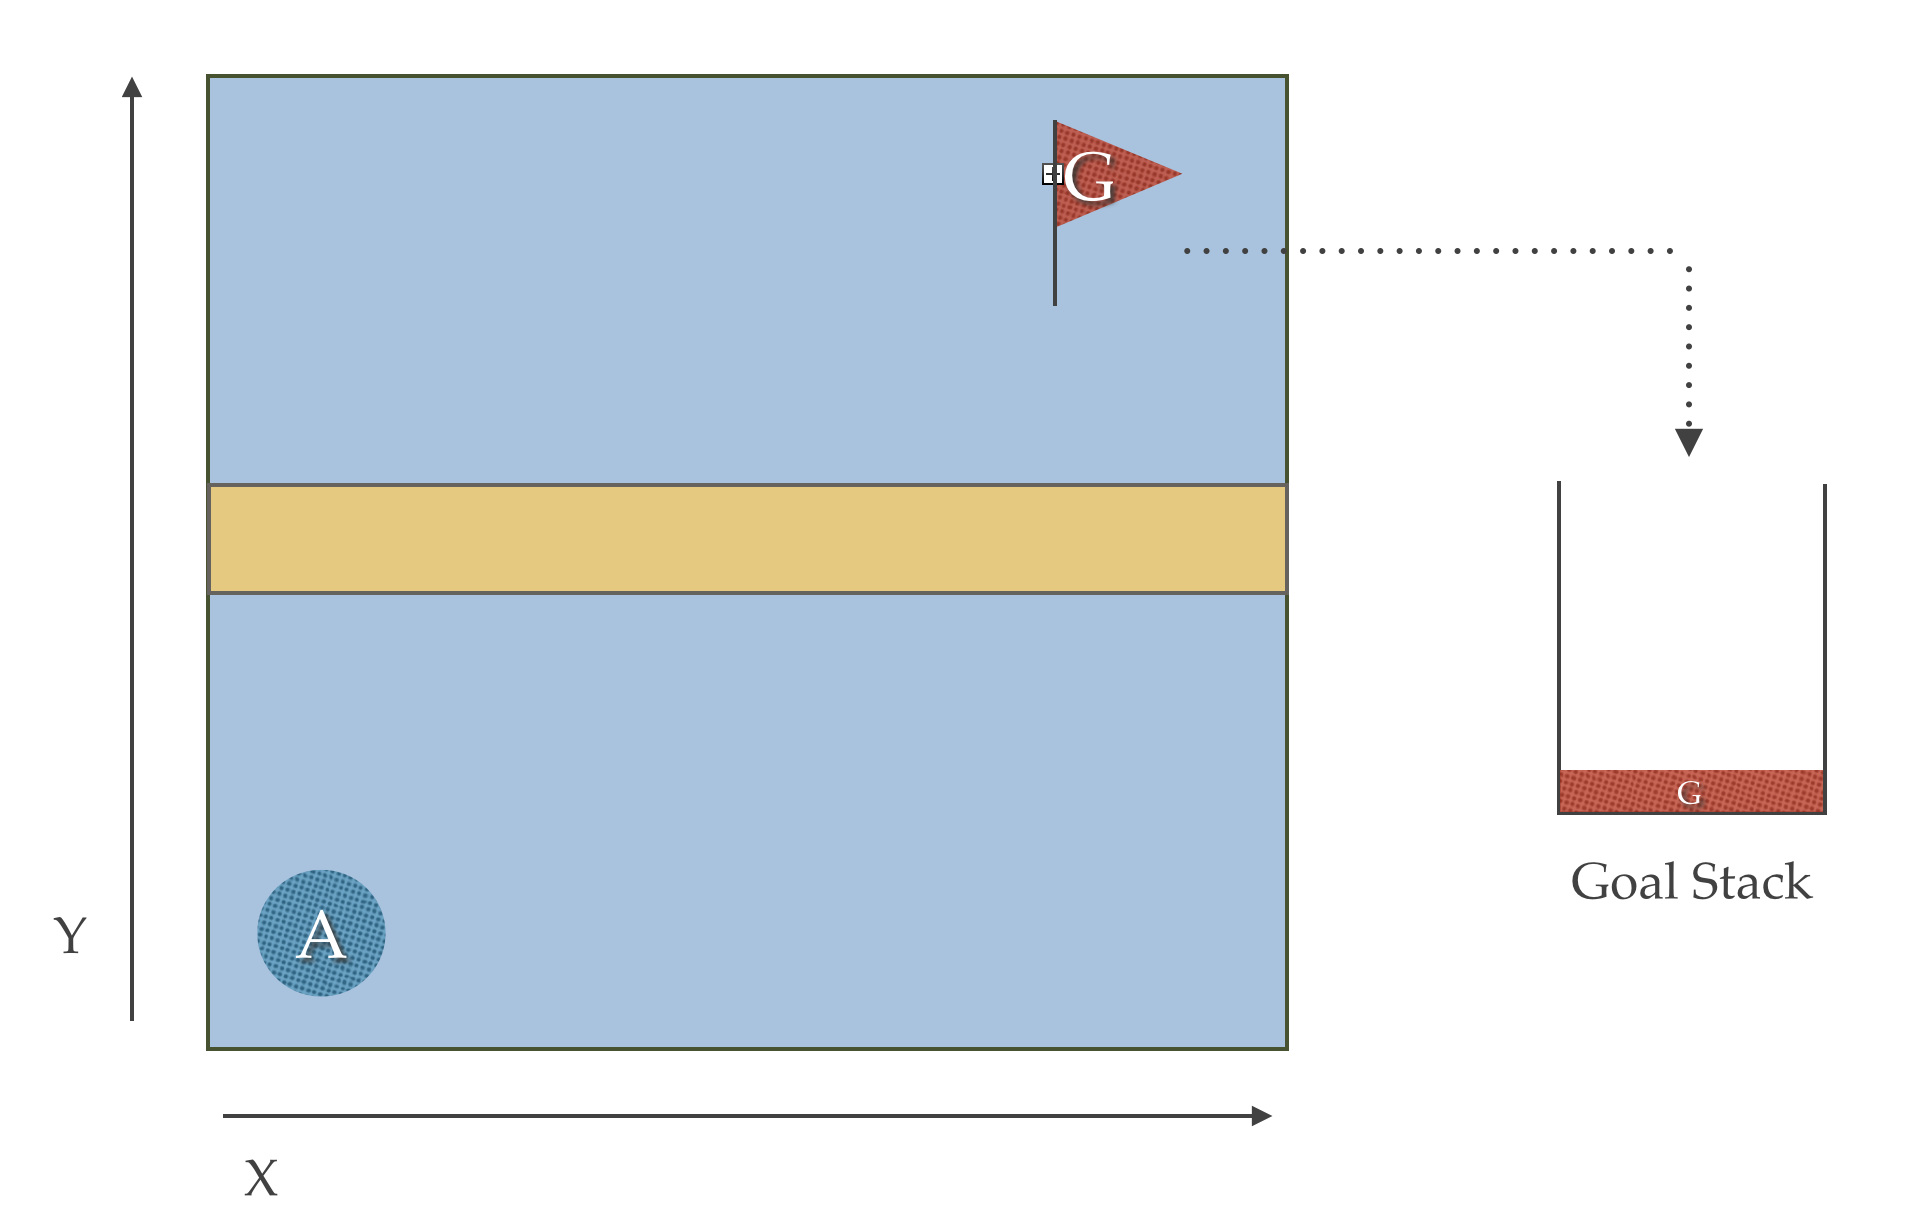
\includegraphics[scale=0.2]{images/problem.png}
	\hspace{19pt}
	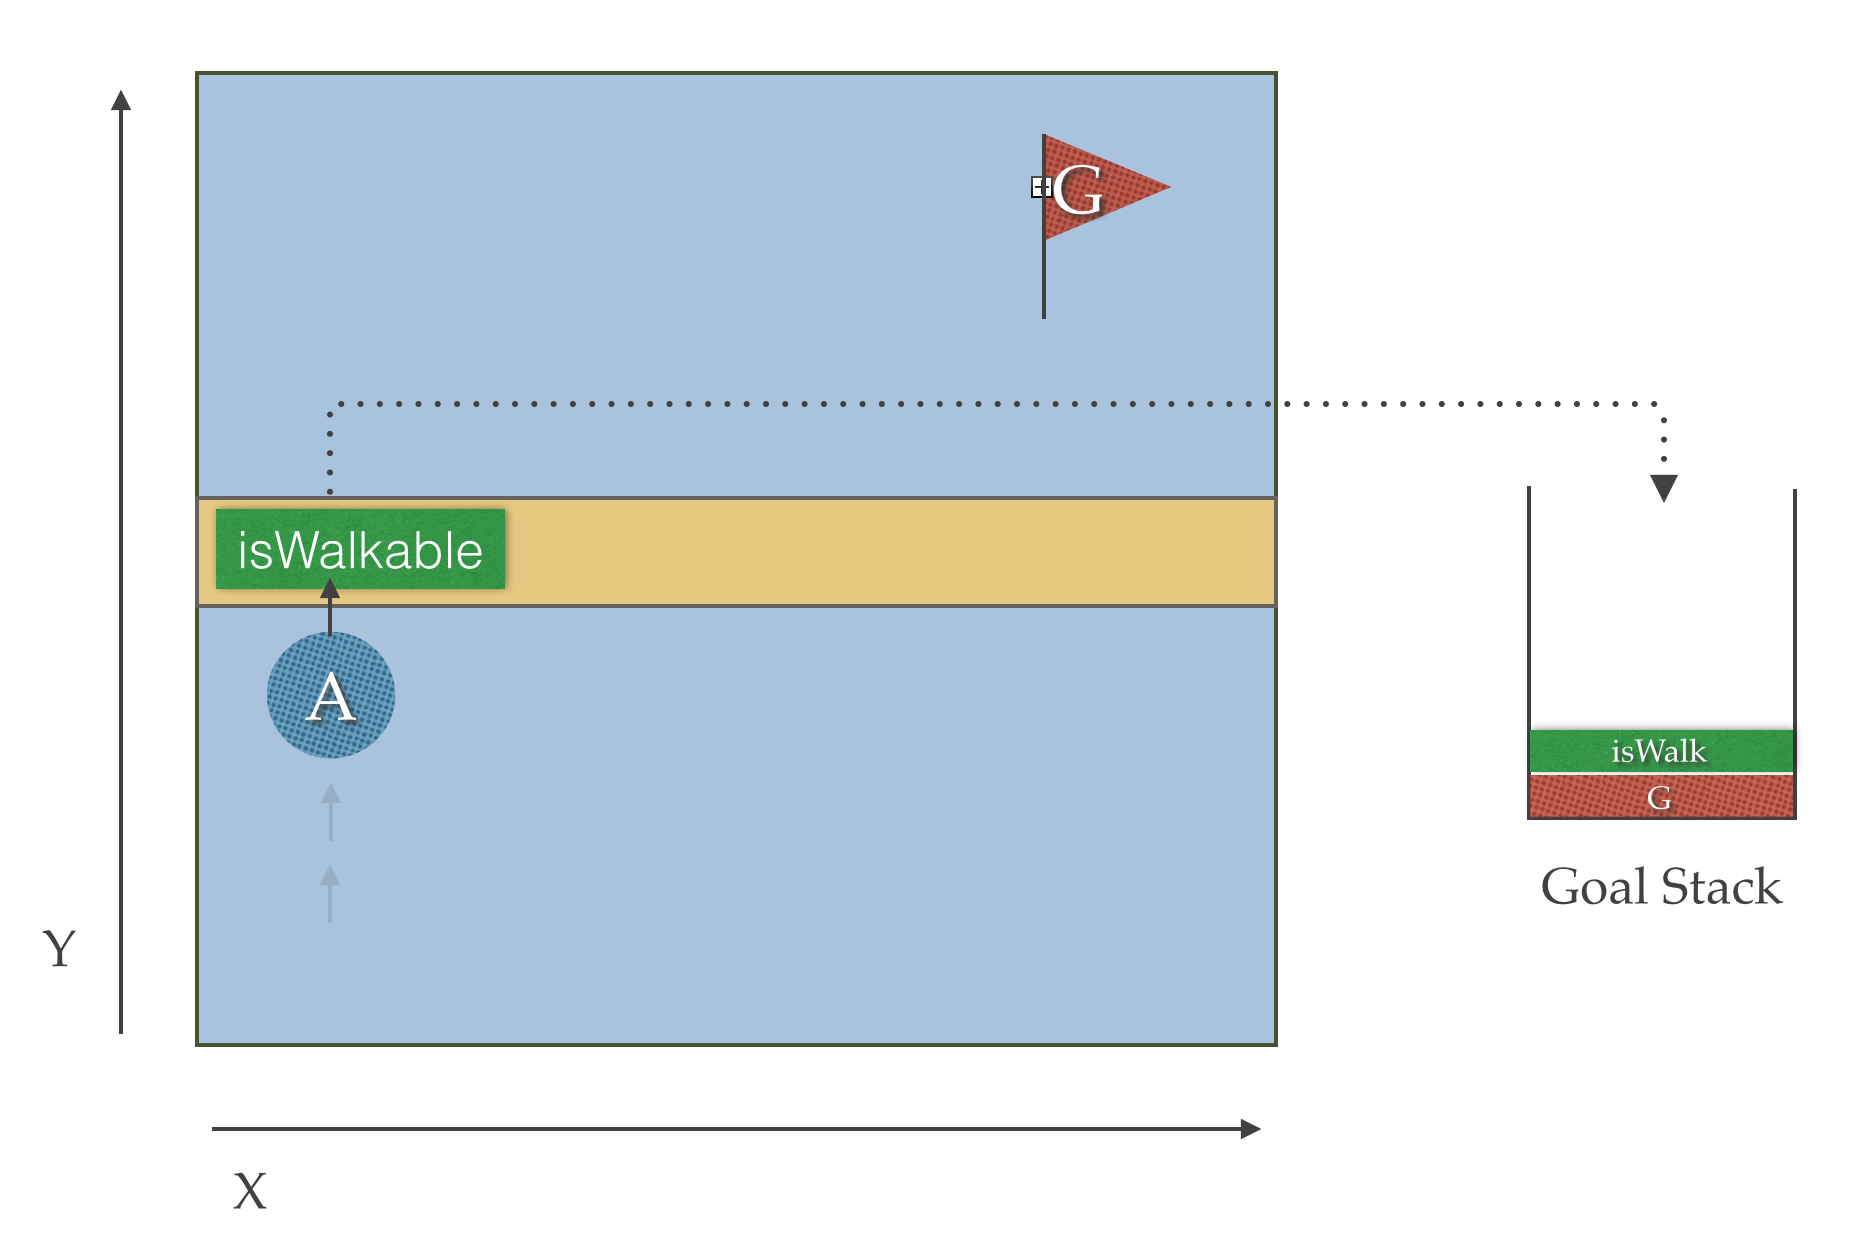
\includegraphics[scale=0.2]{images/isWalk.png}
	\caption{(a) Problem set up and (b) Adding a sub-goal}
	\label{fig:bridgeworld}
\end{figure*}

% Include charts of VI in Minecraft domain.
\section{V. Model}

As discussed previously, our model solves the problem of scaling up to a massive state-action space by pruning both the states and the actions with affordances. Recall that an affordance is what the environment or objects offer an agent, given the agent's current goal. In the context of an MDP, this effectively corresponds to what the {\it actions} allow the agent to achieve, given the agent's goals and the environment. We chose to use subgoal planning as a means of focusing the algorithm toward actions that were reasonable, just like a human might.\footnote{This also parallels a fundamental feature of Gibson's original formulation of affordances - that the affordances that an environment offers an agent are determined in part by the agent's current goal \cite{Gibson}}

Our affordance knowledge is represented as is pictured in Figure (\ref{fig:affordance_tree}), and is composed as a tree, where the root nodes represent propositional functions whose values the agent may change by acting, the non-terminal children are subgoals, and the leaves refer to primitive actions, or pointers to other root nodes. We also maintain a stack that carries the active subgoals of the agent as it is exploring the space. The affordance knowledge need not necessarily be represented as a tree structure - this is merely an appealing visualization that is useful for conceptualizing how the algorithm works.

As we will discuss later, our future work may include changing how our affordance knowledge is represented. Additionally, we assume that the algorithm is given access to perfect affordance knowledge - a knowledge base that is hand crafted by us. At this stage, we are aiming to prove the efficacy of affordance based planning. Once it is clear that affordance based planning promises meaningful gains, then we will target methods for learning these affordances.

The key concept behind our model is that the agent will only look at the appropriate affordances when trying to satisfy a given (sub)goal. This corresponds closely with Gibson's theory of affordances as applied to human cognition, in that, humans only attend to those actions that contribute towards their current goal (i.e. if a human's goal is to break a window, they will automatically search for objects that afford breaking glass, but not consider other irrelevant things). In addition, as the agent encounters new problems it will add subgoals to the Goal Stack, thereby updating what it is current trying to accomplish.

For instance, in our standard bridge building scenario, when the agent reaches the trench, its focus switches from trying to reach the overall goal to simply traversing the trench (and accordingly, it focuses its action search toward those actions that help it traverse trenches, such as building bridges). The combination of dynamically changing the agent's subgoal and only considering affordances relevant to the current subgoal allow us to significantly reduce the search space (even as the complexity and size of the problem ramp up).

\section{VI. Evaluation}

We evaluated our model against Value Iteration in a number of basic path planning scenarios. The most illustrative example is the Bridge World, in which we increment the number of blocks the agent has access to. As the agent is given more blocks it is able to change its environment in more complicated ways (ie. placing multiple blocks in different locations), which causes a combinatorial state-space explosion. These are a good test for the real-world because as we endow a robot with new ways of altering its environment the number of possible states it will be faced with grows rapidly.

As expected, because of the state-space explosion, Value Iteration is unable to handle even moderately complicated scenarios. On the other hand our algorithm is relatively invariant to the complexity introduced by the additional blocks. When testing on a AMD Phenom II X4 955 Processor, Value Iteration took approximately 8 hours to complete the Bridge World scenario with 3 blocks, whereas our algorithm solved the problem almost instantaneously.

As can be seen in Figure (\ref{fig:chart}), giving the agent more blocks causes this problem to be intractable extremely quickly. Our algorithm is capable of solving any basic path planning problem in less then a second, regardless of what other actions are available to it. 

\begin{figure}[h]
\centering
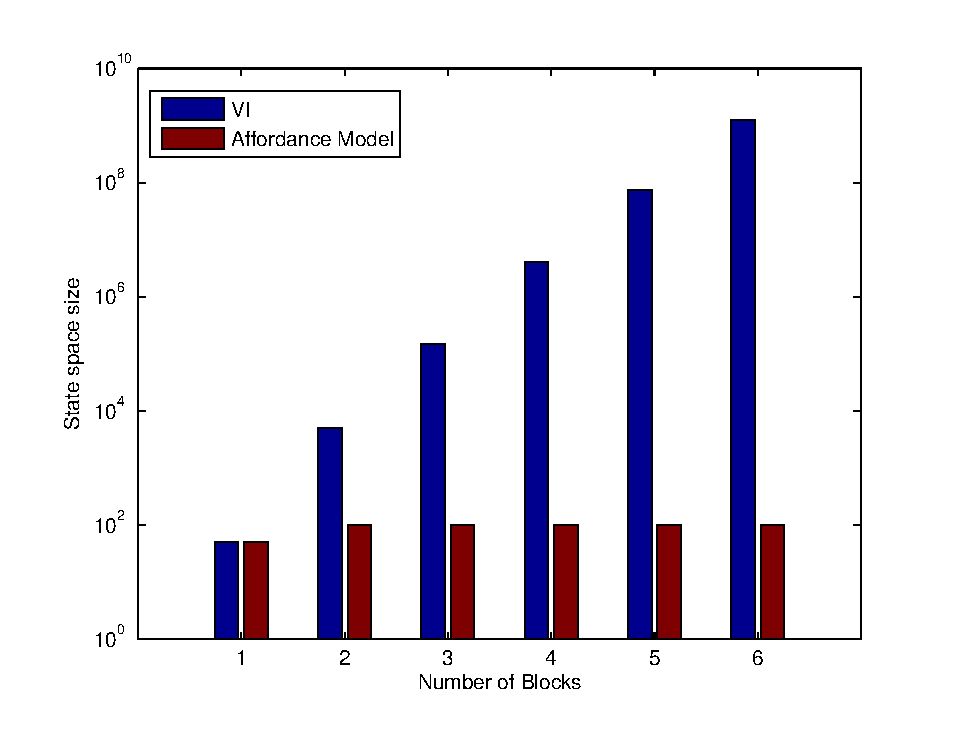
\includegraphics[scale = 0.5]{images/statespace_size}
\caption{Size of State Space in the Two Models \\ (10x10 Bridge World)}
\label{fig:chart}
\end{figure}

This contrasts with Value Iteration, which, when given the full set of actions (adding placement, destruction, jumping, to name a few), will be rendered useless. See Figure (\ref{fig:action_space}) for a visual representation of the action space of our algorithm compared to Value Iteration, when run on a basic Bridge World.

\begin{figure}[h]
	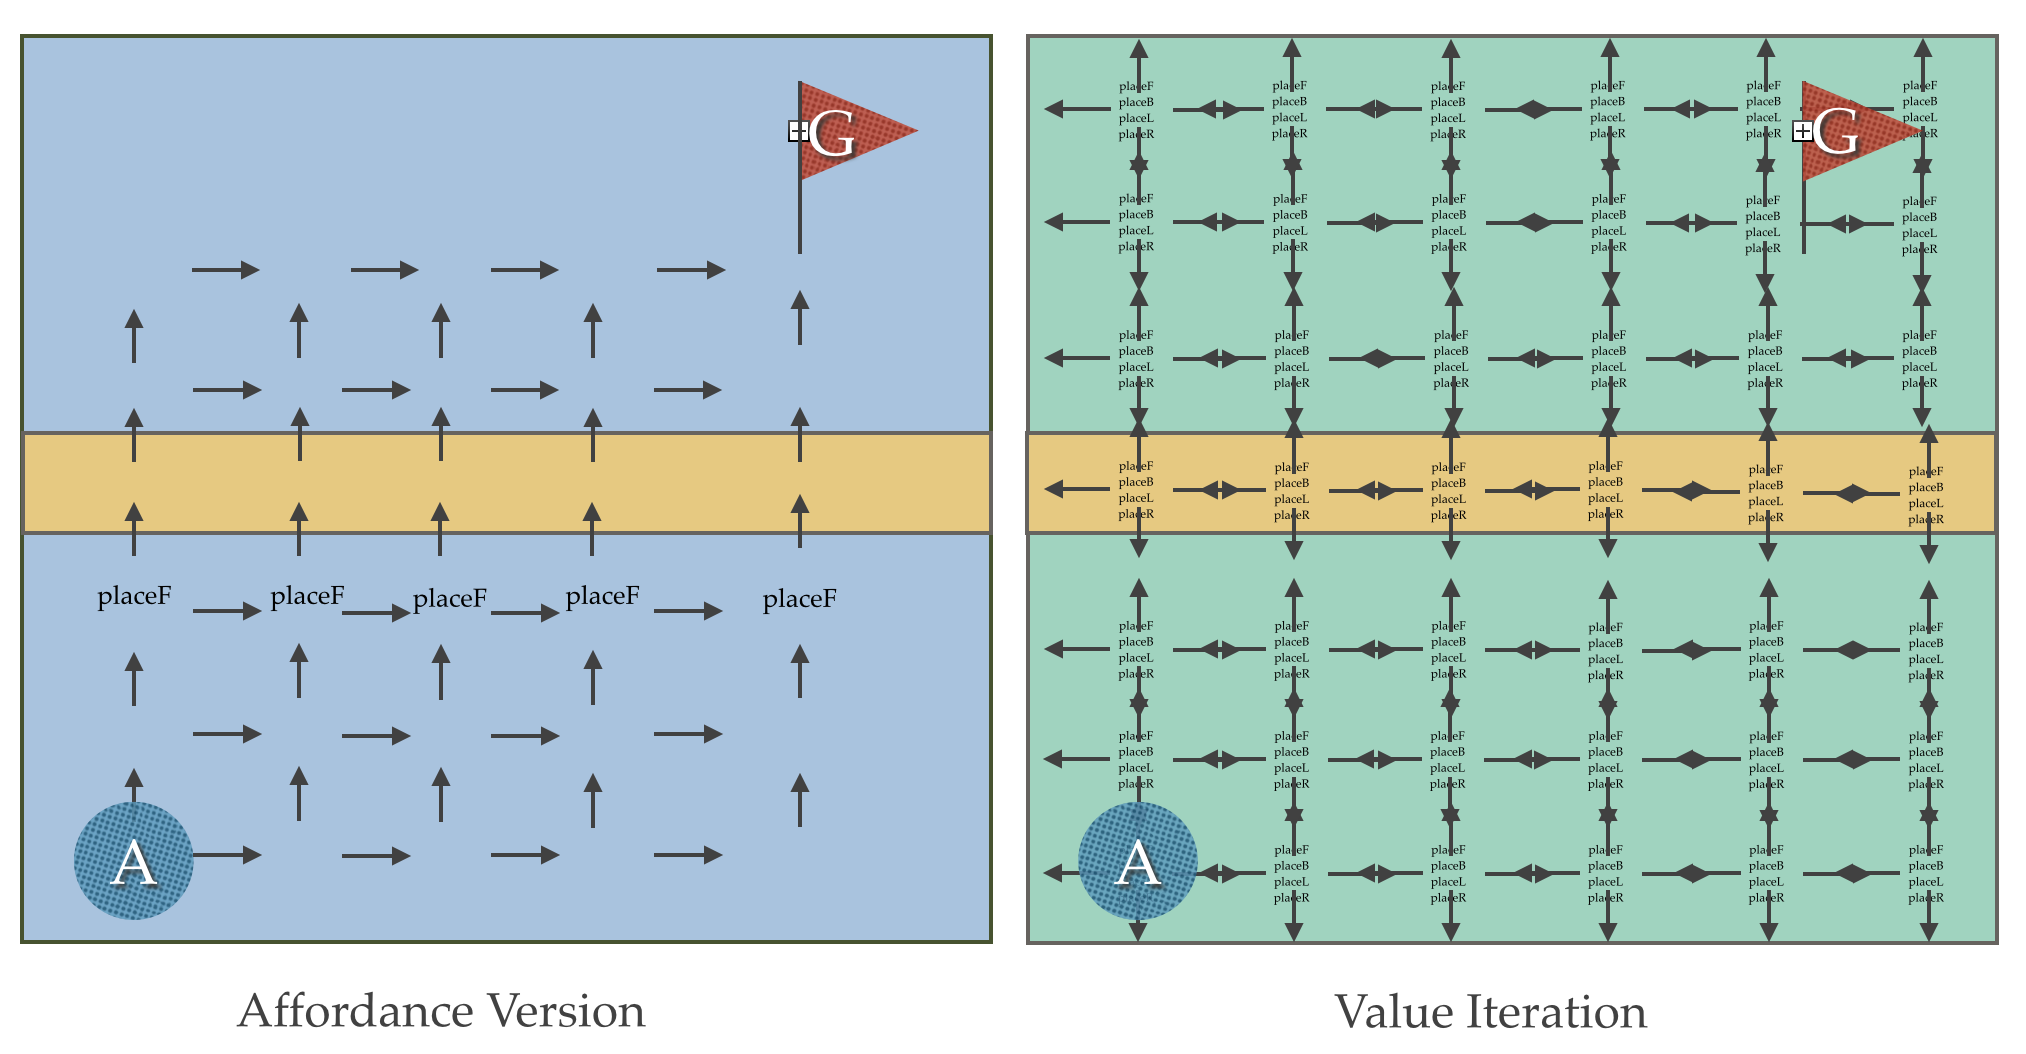
\includegraphics[scale=0.2]{images/comparison.png}
	\caption{Visual layout of the action spaces for our algorithm and Value Iteration}
	\label{fig:action_space}
\end{figure}

%TODO talk bout search over affordance space

\subsection{Scenarios}
Here are a variety of scenarios that we intend to use for experimentation in the Minecraft domain. Value Iteration should be able to handle several of these in their most basic form, however once the agent is able to alter the environment (ie. has a block to place) the state-space explodes and Value Iteration fails. For any of the Building, Tunneling, and Composite tasks, Value Iteration will be forced to enumerate an exploding state-action space, and will fail miserably. We suspect, though, that our algorithm will prove successful in most (if not all) of the following scenarios. We have demonstrated that our algorithm completes all of the path planning tasks listed below in under a second.
\begin{enumerate}
\item Path Planning
\begin{enumerate}
	\item Flat Plane
	\item Walk over a bridge
	\item U-Shaped wall
	\item Indestructible wall with an opening
\end{enumerate}

\item Building
\begin{enumerate}
	\item Build a bridge (of varying length)
	\item Build a block tower (of varying height)
	\item Build other shapes and structures
	\item Build stairs over a wall
\end{enumerate}

\item Tunneling
\begin{enumerate}
	\item Carve a tunnel through a wall
	\item Find an underground goal
	\item Tunnel under an indestructible wall
	\item Find a destructible part of a wall
\end{enumerate}

\item Composite
\begin{enumerate}
	\item Use an elevator to reach the goal
	\item Use a door to get through a wall
	\item Use a ladder to reach the goal
	\item Cross a trench and build a tower with $n$ blocks
	\item Spiraling wall with a mix of doors, tunnels, and bridges
\end{enumerate}
\end{enumerate}
 
One potential problem with our affordance-based planning is that we have simply moved the search from a large state-action space to a much smaller affordance space. This was effectively the concern with Partial Order Planning discussed in Section II. However, as we are currently representing the affordances, the search in this space is linear in the number of edges and vertices of the trees.

Thus, so long as our knowledge base remains relatively compact, the algorithm will have no problem searching across the affordance space. Our intuition is that the knowledge being represented by these affordances is extremely general and may apply across a wide variety of scenarios, and thus, the affordance space should remain relatively small.

% Insert pseudcode
\begin{algorithm}
	\caption{Determines if an action is relevant in a given state, given the current stack of goals}
	\begin{algorithmic}[1]
	\Function{isActRelev}{st, gStack,action}
	\State currAfford $\gets$ getRelAff(st,gStack)
	\State sgs $\gets$ curAff.getSubgoals()
	\While{$\neg$sgs.isEmpty()}
		\State sg $\gets$ sgs.remove()
		\If{sg is true}
			\If{action in sg}
				\Return{true}
			\ElsIf{sg has affordance}
					\State{Determine new subgoal}
					\State{Add new subgoal to sgs}
					\State currAff $\gets$ getRelAff(st,gStack)
					\State sgs $\gets$ curAff.getSubgoals()
			\ElsIf{sg has subgoal and action in subgoal}
				\State \Return true
			\EndIf
		\EndIf
	\EndWhile
	\State \Return{false}
	\EndFunction
	\end{algorithmic}
\end{algorithm}

We have included pseudo code of the primary component of our algorithm that determines if an action is relevant in a particular state, given the current goal stack (See Algorithm 1). The algorithm is called within a reachability analsysis, that typically enumerates all of the states in order to optimize Value Iteration. Instead, we only enumerate those states that are reachable from applications of 'relevant' actions, as determined by Algorithm 1.

\section{VII. Conclusion}
In this paper, we introduced an approach to planning around the classic Sequential Decision Making problem structure that integrated the concept of an affordance into the versatile but limited algorithm, Value Iteration. We have demonstrated where the classical version of Value Iteration falls short, and proven empirically that our own version is capable of tackling the scale and complexity needed from a planning algorithm, at least in the few path planning tasks we visited.

\section{VIII. Future Work}
\subsection{Prove Generality}
We have a long way to go in order to prove the generality of this knowledge - as of right now, we have simply proven that it is capable of scaling to problems in Minecraft with arbitrarily many blocks. A large next step for this project is to empirically validate the generality of the affordance-based knowledge representation we have proposed by scaling the system to solve other more complicated scenarios.

Even though we have not yet fully implemented the system across a wide variety of scenarios, given how it performed on the Bridge World scenario, we strongly suspect that it will deal with other planning task types, too. We have compiled a list of future scenarios that we believe are solvable by our affordance-based approach to planning, assuming the algorithm is given access to perfect affordance knowledge (i.e. a human overseer provides a knowledge base from the get go).

% Using affordances to plan
\subsection{Learning}
This points to another fundamental issue with our project at this stage - it requires a hefty amount of information in order to solve problems. Furthermore, this information is not obvious - to the untrained overseer, it is not clear what affordances are necessary to solve a particular task. Therefore, one of the primary next steps for this project is to develop a learning technique that will automatically generate these affordances. This document is intended to demonstrate the efficacy of the algorithm, once it has all the affordance knowledge it needs.

\subsection{Additional Baselines}
An additional next step is to prove, decisively, that pruning both the state {\it and} action spaces is necessary in order to achieve optimal scalability and robustness - we have merely hypothesized about the shortcomings of subgoal planning (i.e. Branavan's work in Minecraft), but have not empirically validated these theories. We also need to prove that our model is capable of solving the same problems that Branavan's subgoal planner was able to solve (e.g. baking bread given subgoal knowledge about the constituents that are required in order to make bread) \cite{Branavan2012}.

Another thing we ought to do in the future is compare our algorithm against some additional baselines, including a random planner, an RRT \cite{LaValle1998}, A* with a meager attempt at creating a decent (likely non-admissible) heuristic\footnote{Or at least determine that coming up with an admissible heuristic for A* in many non-path planning domains is extremely difficult if not impossible}, STRIPS/PDDL/FF, Policy Gradient and other Policy Approximation methods. We also want to verify that planners that leverage Macroactions or Options do not guarantee better or comparable performance.

\subsection{Natural Language}
The final extension to consider is how language may be tied to affordances - there is something fundamental tying affordances with language, and specifically, with object classification. For instance, consider the bridge example discussed above - any object that provides passage over an impass may be considered a bridge; a bridge is defined precisely by the fact that it affords passage. Since our formalism is relatively easy to understand for a human, we expect there to be additional extensions for natural language processing and possibly dialogue systems, in which natural language may be mapped directly to affordance knowledge.

\section{VIII. Acknowledgments}
We would like to thank the following people for their interest, inspiration, guidance, and support throughout this project! \\ \\
Stefanie Tellex,  Eugene Charniak, The entire Fall 2013 CS2951 class, The H2R group @ Brown, James MacGlashan for his extensive work on BURLAP and his assistance with the project, Yoav Artzi, Nate Kushman, Brown Robotics.\cite{Branavan2012}

\bibliography{afford}
\bibliographystyle{aaai}

\end{document}